%Übersicht ist in getrennter Datei webseiten-uebersicht.
\paragraph{Vertiefung} 
Das Internet verbindet weltweit verschiedene Computer-Netzwerke. Systeme wie das WWW als Internetdienst ermöglichen dabei den Austausch der Daten. Das WWW selbst ist wiederum ein System aus Hypertexten und Hypermedia im Internet, das via HTTP als Protokoll kommuniziert. Eine Webseite ist in der Regel eine HTML-Datei mit Verweisen, die als Hyperlinks entweder auf andere Stellen im selben Dokument oder auf beliebig viele weitere Ressourcen im WWW verweist. Webseiten bilden die einzelnen Bestandteile einer Website und können sowohl als Homepage (resp. Startseite) als auch in Form jeder beliebigen anderen Seite innerhalb einer Website enthalten sein. Webseiten als HTML-Dokumente können nicht ausschließlich nur im WWW auftreten, sondern etwa auch lokal vorliegen.

\subparagraph{Grundsätzliche Funktionsweise} Das generelle Vorgehen zum Abrufen einer Webseite in Form einer HTML-Datei kann schematisiert wie folgt beschrieben werden: Nach dem Öffnen des Webbrowsers (1) erfolgt die Eingabe der URI (z.B. \url{http://www.ianus-fdz.de/}) bzw. der Klick auf einen Hyperlink (2). Dies bewirkt, dass der Webbrowser anhand der in der URI enthaltenen Domain (z.B. www.ianus-fdz.de) die Internet Protocol (IP) Adresse von einem Domain Name System (DNS) Server bezieht (3); den Datenaustausch regelt das Transmission Control Protocol (TCP). Jedes Gerät, mit dem eine Internetverbindung hergestellt werden kann, verfügt über eine IP-Adresse, die eine eindeutige Identifikation des Gerätes ermöglicht. Anhand der IP-Adresse fragt nun der Webbrowser als Web-Client um das gewünschte HTML-Dokument beim entsprechenden Web-Server, auf dem das Dokument gespeichert ist, an (4). Der Web-Server stellt nun das angeforderte HTML-Dokument zur Verfügung (5), welches vom Webbrowser empfangen (6) und dargestellt wird (7). Siehe dazu auch Abbildung \ref{abb:webseiten-aufbau}.

Dies ist nur ein grundsätzlicher Überblick hinsichtlich der wichtigsten Elemente. Ausführlichere Informationen finden sich auf \url{https://wiki.selfhtml.org/wiki/Grundlagen}. Zur Geschichte des Internets und WWW existieren zahlreiche Abhandlungen, siehe hierfür etwa detailliert \url{https://wiki.selfhtml.org/wiki/Grundlagen/Entstehung_des_Internet}.

\tikzset{
		%Define standard arrow tip
    >=stealth',
		% Define arrow style
    pfeil/.style={
           ->,
           draw=ianusBlau, very thick,
           shorten <=0.8em,
           shorten >=0.8em
					},
    %Define style for boxes
		abgerundetAussen/.style={
           rectangle,
           rounded corners,
           draw=ianusBlau, very thick,
					 inner xsep=0.5em,
					 minimum height=3em,
					 minimum width=10em,
           text centered	
					},
    abgerundet/.style={
           rectangle,
           rounded corners,
           draw=ianusGrau, very thick,
					 fill=ianusGrau,
           minimum height=2em,
           text centered}
}
\begin{figure}[!hpt]
	\begin{center}
	\begin{tikzpicture}[remember picture, node distance=1cm, auto]
		\node[abgerundetAussen] (browser) {
			\begin{tikzpicture}
				\node[abgerundet] (url) {http://www.ianus-fdz.de};
				\node[right =-1.5cm of url] (2) {(2)};
				\node[abgerundet, below =1.5cm of url] (inhalt) {
\includegraphics[width=.4\textwidth]{bilder/webseiten_ianus.png}};
				\node[above right =-1cm and -1.5cm of inhalt] (7) {(7)};
			\end{tikzpicture}
		};
		\node[above left =-0.5cm and 0.1cm of browser] (1) {(1)};
		\node[abgerundetAussen, below left =2cm and -3cm of browser] (dns) {
			\begin{tikzpicture}
				\node[] (dnsserverLabel) {DNS-Server};
			\end{tikzpicture}
		};
		\node[below left =0cm and -0.5cm of dns] (3) {(3)};
		\path[->, pfeil] (browser) edge [bend left=10] node {Domain} (dns);
		\path[->, pfeil] (dns) edge [bend left=10] node {IP} (browser);
		\node[abgerundetAussen, below right =2cm and -2cm of browser] (server) {
			\begin{tikzpicture}
				\node[] (serverLabel) {Server};
				\node[below =0cm of serverLabel] (ip) {IP: 134.95.80.147};
				\node[abgerundet, below =0cm  of ip] (dok1) {Dokument X};
				\node[abgerundet, below =0cm  of dok1] (dok2) {Dokument Y};
				\node[abgerundet, below =0cm  of dok2] (dok) {...};
			\end{tikzpicture}
		};
		\node[below left =0cm and -0.8cm of server] (4,5) {(4,5)};
		\path[->, pfeil] (browser) edge [bend left=20] node {IP} (server);
		\path[->, pfeil] (server) edge [bend right=10] node {Dokument} (browser);
		\node[below right =0.2cm and -1.7cm of browser] (6) {(6)};
	\end{tikzpicture}
	\end{center}
	\caption{In dem Webbrowser (1) erfolgt die Eingabe der URI oder der Klick auf einen Hyperlink (2). Der Webbrowser bezieht die IP-Adresse vom DNS-Server (3). Mit der IP-Adresse wird beim entsprechenden Web-Server das gewünschte Dokument angefragt und zur Verfügung gestellt (4,5). Das angeforderte Dokument wird vom Browser empfangen (6) und dargestellt (7).}
	\label{abb:webseiten-aufbau}
\end{figure}

\subparagraph{Webbrowser}
Ein Webbrowser ist ein Computerprogramm zum Abrufen sowie Darstellen von Ressourcen (HTML-Dokumente, multimediale Inhalte, ganze Webanwendungen etc.) und ist die Schnittstelle zwischen dem Nutzer und dem WWW. Er ermöglicht das sequenzielle Abrufen und Betrachten von Webseiten unter Verwendung von Hyperlinks im WWW (surfen), wobei es keine Rolle spielt, ob eine anzuzeigende Ressource über das WWW oder lokal zur Verfügung gestellt wird. Für die Darstellung der Ressourcen können Plug-ins herangezogen werden. Ein Webbrowser ermöglicht zudem die Speicherung von Dateien und Programmen aus dem Internet auf dem Computer. Heutige Webbrowser unterstützen die Anzeige mehrerer Fenster gleichzeitig in Form von Tabs (Registerkarten, Reiter). Beliebte aktuelle Webbrowser sind Google Chrome, Mozilla Firefox, Microsoft Internet Explorer, Apple Safari und Opera: \url{http://www.w3schools.com/browsers/}

\subparagraph{URIs}
Uniform Resource Identifiers (URI, einheitlicher Bezeichner für Ressourcen) ermöglichen die Identifikation einer Ressource (z. B. einer Webseite oder eines PDF-Dokumentes) im Internet. Im Bereich des WWW treten URIs vor allem als Uniform Resource Locators (URL, einheitlicher Quellenanzeiger, also die eigentlichen "`Internetadressen"', z. B. \url{http://www.ianus-fdz.de/}) undUniform Resource Names (URN, einheitlicher Name für Ressourcen) auf: URLs definieren dabei im WWW den Ort einer Ressource, URNs benennen die Ressource selbst. Eine URN kann mit einer oder mehreren URLs verknüpft sein, etwa wenn dieselbe Ressource an verschiedenen Speicherorten verfügbar ist. Unter anderem verwenden Nationalbibliotheken URNs als Persistente Identifikatoren zur Kennzeichnung von Onlinepublikationen: Die Deutsche Nationalbibliothek hat beispielsweise das Dokument "`Policy für die Vergabe von URNs im Namensraum urn:nbn:de"' mit der URN <urn:nbn:de:101-2012121200> ausgestattet. Man benötigt für gewöhnlich einen URN-Resolver, der die zum URN gehörige(n) URL(s) anzeigt, um an die gewünschte Ressource zu gelangen. Die Deutsche Nationalbibliothek bietet einen solchen unter der URI http://nbn-resolving.org/ an, wo für die URN <urn:nbn:de:101-2012121200> (= "`Name"')  die URL http://d-nb.info/1029114455/34 (= "`Adresse"') angegeben wird. Detaillierte Informationen zu URIs, URLs, URNs und persistenten Identifikatoren sind in dem "`Abschlussbericht Testbed 'Persistent Identifiers'"'\footnote{\url{http://www.ianus-fdz.de/attachments/download/560/Testbed-Persistent\%20Identifiers.pdf}} zu finden.

\subparagraph{Webseiten} 
Unter der Verwendung von HTML, CSS, JavaScript sowie weiteren Ressourcen, z. B. Rastergrafiken, Vektorgrafiken, Video- oder Audiodateien werden Webseiten erstellt. Die einzelnen Ressourcen können in verschiedenen Ordnern oder sogar an verschiedenen Orten liegen. Eine Webseite besteht hierbei aus drei grundsätzlichen Schichten: der Struktur, dem Layout und dem Verhalten. Die Struktur bzw. der Aufbau wird durch HTML organisiert, CSS definiert das Layout der Webseite und JavaScript bestimmt, wie sich die Webseite bei Interaktionen des Nutzers verhält. Weitere Informationen dazu finden sich auf \url{https://wiki.selfhtml.org/wiki/HTML/Tutorials/Trennung_von_Inhalt,_Pr\%C3\%A4sentation_und_Verhalten} 

\subparagraph{HTML}
Bei Hypertext Markup Language (HTML) handelt es sich um eine Auszeichnungssprache, durch die Dokumente strukturiert beschrieben werden können. HTML kann zur Erstellung von Webseiten aber auch zur Erstellung von lokalen Dokumenten verwendet, ausgedruckt oder mit Hilfe synthetischer Stimmen barrierefrei für Menschen mit Sehbeeinträchtigungen auf Audio-Systemen ausgegeben werden. Webbrowser visualisieren die Auszeichnungsbefehle unter eventueller Berücksichtigung von CSS-Dateien und machen so das Dokument menschenlesbar. Ein Kernelement von HTML ist die Verfügbarkeit von Verweisen in Form von Hyperlinks, durch die andere Stellen im selben Dokument, aber auch andere Ressourcen im WWW und im Internet aufgerufen werden können. 

Der aktuelle Standard für HTML-Dateien ist HTML5 und wird mit einer Dokumenttypdeklaration am Beginn der HTML-Datei angegeben. Da HTML im ASCII-Zeichensatz verfasst wird, eignen sich Text-Editoren bzw. spezialisierte HTML-Editoren zur Bearbeitung. HTML5 verwendet als Standardzeichensatz UTF-8, was auch beibehalten werden sollte.

Das Grundgerüst einer HTML Datei besteht aus:
\begin{itemize}
	\item Der Dokumenttypdeklaration in der Form <!DOCTYPE html> für HTML5.
	\item Dem HTML-Wurzelelement <html>, welches den Inhalt der HTML-Datei umklammert. 
	\item Dem Kopfelement <head>, welches die Kopfdaten (z.B. das verpflichtende Titelelement) beinhaltet. Auch ist hier der geeignete Ort für allgemeine Kommentare zum HTML Dokument (z.B. Metadaten). Die Kopfdaten werden im Browser nicht angezeigt. 
	\item Dem Titelelement <title> als Teil des <head>, welches verpflichtend anzugeben ist. 
	\item Dem Körperelement <body>, das den anzuzeigenden Inhalt enthält. 
\end{itemize}

Dieser Aufbau gestaltet sich in HTML folgendermaßen: 

\lstset{language=HTML}
\begin{lstlisting}[frame=L, xleftmargin=1.5\parindent, rulecolor=\color{ianusGrau}]
<!DOCTYPE html>
<html>
	<head>
		<title></title>
    <!-- Kommentare -->
	</head>
	<body>
		anzuzeigender Inhalt
	</body>
</html>
\end{lstlisting}



Bei HTML-Dokumenten können zusätzliche Informationen wie z.B. Metadaten als Kommentare an beliebiger Stelle eingegeben werden, wie etwa der <head>-Bereich. Kommentare werden durch die Zeichenfolge <!-- eingeleitet und durch die Zeichenfolge --> abgeschlossen. Sie werden von einem Webbrowser generell nicht angezeigt, können jedoch mittels eines Texteditors dargestellt werden.

Ein kurzes Beispieldokument mit rudimentären Metadaten in HTML, das in einem Webbrowser den Text "`Testüberschrift: Dies ist ein einfaches Beispiel"' anzeigt, könnte wie folgt aussehen: 
\lstset{language=HTML}
\begin{lstlisting}[frame=L, xleftmargin=1.5\parindent, rulecolor=\color{ianusGrau}]
<!DOCTYPE html>
<html>
	<head>
		<meta charset="utf-8">
		<meta name="description" content="Ein Beispieldokument">
		<meta name="keywords" content="example, html, dai, ianus">
		<meta name="author" content ="Dominik Hagmann">
		<title>Beispieldokument</title>
		<!-- Weitere Metadaten: Erstellt: 11.2016, Lizenz: CC-BY -->
	</head>
	<body>
		<h1>Testüberschrift: </h1>
		<p>Dies ist ein einfaches Beispiel.</p>
	</body>
</html>
\end{lstlisting}


\subparagraph{CSS}
Cascading Style Sheets (CSS) dienen zur Formatierung von HTML- und XML-Dokumenten. HTML-Dokumente besitzen einige vom jeweiligen Browser vorgegebene Formatierungen, etwa hinsichtlich der Gestaltung der Überschriften oder der Hyperlinks. Mittels CSS können deutlich umfangreichere Designs erzeugt werden; CSS-Dateien, die die Formatierung regeln, sind für professionelles Web-Design von höchster Bedeutung. CSS ermöglicht die Formatierung aller HTML-Elemente sowie zahlreicher weiterer Bestandteile, die nicht in HTML enthalten sind. Wahlweise kann mittels CSS global das gesamte Design auf einmal bestimmt oder aber auch die Formatierung einzelner HTML-Objekte individuell definiert werden. Für CSS eignen sich dieselben Editoren wie für HTML. 

Durch einen Selektor wird in der CSS-Datei ein Element angewählt und der Wert der Eigenschaft definiert. Dies geschieht in der Form "`Selektor \{Eigenschaft : Wert; \}"'. Folgendes Beispiel färbt alle Buchstaben eines Absatzes blau ein:
\lstset{language=HTML}
\begin{lstlisting}[frame=L, xleftmargin=1.5\parindent, rulecolor=\color{ianusGrau}]
p {color: blue; }
\end{lstlisting}


\subparagraph{JavaScript}
Bei JavaScript (nicht zu verwechseln mit den Programmiersprachen Java und JScript) handelt es sich um eine Implementation der Skriptsprache ECMAScript und ist die am weitesten verbreitete Programmiersprache für Webseiten. Mittels JavaScript können Webseiten um Zusatzfunktionen ergänzt werden. Dabei kann der JavaScript Code abhängig von dessen Einsatzzweck direkt in der HTML-Datei im Head oder Body eingebettet oder in einer separaten Datei mit der Endung .js vorhanden sein. Allgemein empfiehlt es sich, JavaScript extern als js-Datei zu speichern und in dem HTML-Dokument mittels einer Skriptreferenz darauf zu referenzieren. 

JavaScript stattet Webseiten mit Elementen aus, durch die der User mit der Webseite interagieren kann. Ein Beispiel für eine solche Interaktion auf einer Webseite ist, per Mausklick auf einen Button den Inhalt von Textabschnitten zu ändern: \url{http://www.w3schools.com/js/tryit.asp?filename=tryjs_whereto_head}. In diesem Beispiel ist das Skript in HTML eingebettet:
\pagebreak
\lstset{language=HTML}
\begin{lstlisting}[frame=L, xleftmargin=1.5\parindent, rulecolor=\color{ianusGrau}]
<!DOCTYPE html>
<html>
	<head>
		<script>
			function myFunction() {
				document.getElementById("Beispiel").innerHTML=
					"... der nun verändert wurde ;-)";
			}
		</script>
	</head>
	<body>
		<h1>Beispiel zu JavaScript</h1>
		<p id="Beispiel">Dies ist der ursprüngliche Text...</p>
		<button type="button" onclick="myFunction()">
			Bitte drücken
		</button>
	</body>
</html>
\end{lstlisting}

Ist der Code in einer separaten Datei gespeichert, benötigt man eine Skriptreferenz: 
\lstset{language=HTML}
\begin{lstlisting}[frame=L, xleftmargin=1.5\parindent, rulecolor=\color{ianusGrau}]
<script src="Beispielskript.js"></script>
\end{lstlisting}

Aufgrund des Umfangs wird nicht weiter auf JavaScript im Speziellen eingegangen. Weiterführende Informationen finden sich beispielsweise auf \url{https://wiki.selfhtml.org/wiki/JavaScript/Tutorials/Einf\%C3\%BChrung}


\subparagraph{Dynamische Websites}
Wenn die angezeigten Inhalte einer Webseite aus einer zugrunde liegenden Datenbank stammen, handelt es sich um eine dynamische Webseite. Bei dem Besuch einer dynamischen  Webseite wird also nicht ein fertiges statisches HTML-Dokument abgerufen, sondern ein anzuzeigendes HTML-Dokument wird ad-hoc und individuell aus den Einträgen in der Datenbank generiert. Mit Hilfe von Content-Management-Systemen (CMS), wie beispielsweise Joomla, Drupal, TYPO3 oder WordPress, können die Inhalte solcher Websites auch ohne HTML-Kenntnisse verwaltet und gepflegt werden.

Für die Archivierung von vollständigen CM-Systemen gelten umfangreichere Anforderungen, als bei der Archivierung einzelner, zum Zeitpunkt des Aufrufes, statischer Webseiten daraus. Es muss beispielsweise entschieden werden, ob der gesamte Funktionsumfang der Website oder lediglich die darin enthaltenen Informationen gesichert werden sollen.


\paragraph{Praxis} 
In diesem Abschnitt werden Programme und Editoren vorgestellt, um eine Webseite zu bearbeiten.  Neben einer allgemeinen Übersicht der Archivierungsmöglichkeiten, wird auf die verschiedene Möglichkeiten eingegangen, um Webseiten als PDF, MHTML, MAFF oder HTML mit Data-URIs zu archivieren. Auch Archivierungsmöglichkeiten für gesamte Websites werden vorgestellt, sowie einige Hinweise zu Screenshots gegeben. Zahlreiche Hinweise finden sich auch im Praxisabschnitt des Kapitels Textdokumente ab Seite \pageref{textdokumente}.

\subparagraph{Editoren}
Um HTMl, CSS und JavaScript Dateien von Webseiten zu bearbeiten, wird ein Texteditor benötigt. Eine ausführliche Übersicht bietet der Abschnitt Praxis im Kapitel Textdokumente. Zusätzlich zu den dort besprochenen Editoren existieren spezielle Editoren für das Webdesign, unter Umständen mit WYSIWYG-Modi, bzw. mächtige Code-Editoren, die umfangreiche Möglichkeiten zur Codeerstellung bieten, jedoch oftmals auch das nötige Hintergrundwissen hinsichtlich der verwendeten Sprache und deren Syntax verlangen. Ein Beispiel für einen WYSIWYG-Editor ist Adobe Muse CC, Beispiele für professionelle Code-Editoren sind Adobe Dreamweaver CC und Sublime Text von Jon Skinner wobei es sich jeweils um proprietäre Softwarelösungen handelt. Die Systeme von Adobe sind für Windows und Mac OS verfügbar, Sublime Text zusätzlich für Linux. 

Frei verfügbare Alternativen stellen Aptana Studio, SeaMonkey und  BlueGriffon dar, die alle für Windows, Mac OS und Linux verfügbar sind. Aptana Studio bietet Werkzeuge zur Erstellung von HTML, CSS und JavaScript. SeaMonkey und BlueGriffon haben einen WYSIWYG-Editor.

\begin{flushleft}
	Adobe Muse CC: \urllist{https://www.adobe.com/at/products/muse.html}
	Adobe Dreamweaver CC: \urllist{https://www.adobe.com/at/products/dreamweaver.html}
	Sublime Text: \urllist{https://www.sublimetext.com}
	Aptana Studio: \urllist{http://www.aptana.com}
	Seamonkey: \urllist{http://www.seamonkey-project.org}
	BlueGriffon: \urllist{http://www.bluegriffon.org}
\end{flushleft}


\subparagraph{Archivierungsmethoden}

Die Archivierung einer Webseite wird schnell und einfach durch ihre Konvertierung in eine PDF-Datei und anschließende Speicherung als PDF/A-Datei bewerkstelligt. Sie kann auf unterschiedliche Weise mittels des Webbrowsers, durch eigene Online-Konvertierungsdienste oder spezielle Softwareprogramme erfolgen. 

Alternativ kann eine Speicherung und Archivierung der Webseite als HTML-Datei mit Data URIs, MHTML-Datei oder MAFF-Container vorgenommen werden. Hierbei ist zu beachten, dass nicht alle Webbrowser alle Formate unterstützen bzw. ein vorhergehendes Entpacken der komprimierten Webseite nötig ist. Eine Übersicht der unterstützten Formate für aktuelle Webbrowser ist in Tabelle \ref{tab:webseiteOeffnen} und Tabelle \ref{tab:webseiteSpeichern} gegeben.

\begin{table}[hbt]
\centering
\footnotesize
\begin{tabular}{lcccc}
	\toprule
	Webbrowser	& Data-URI & MAFF & MHTML & PDF \\
	\midrule
	Chrome (54.0.x) & \checkmark & (\checkmark)\textsuperscript{*} & \checkmark & \checkmark \\
	Edge & \checkmark & (\checkmark)\textsuperscript{*} & \boldmath$\times$ & \checkmark \\
	Firefox (49.0.x) & \checkmark & \checkmark & (\checkmark)\textsuperscript{**} & \checkmark \\
	Internet Explorer (11.x) & \checkmark & (\checkmark)$^*$ & \checkmark & \checkmark \\
	Opera (40.0.x) & \checkmark & (\checkmark)\textsuperscript{*} & \checkmark & \checkmark \\
	Safari (10.0.x) & \checkmark & (\checkmark)\textsuperscript{*} & (\checkmark)\textsuperscript{**} & \checkmark \\
	Vivaldi (1.4.x) & \checkmark & (\checkmark)\textsuperscript{*} & \checkmark & \checkmark \\
	\midrule
	\multicolumn{5}{l}{ \textsuperscript{*}vorheriges Entpacken \textsuperscript{**}PlugIn benötigt}\\

	\bottomrule 
\end{tabular}
\caption{Überblick über die näher behandelten Speichermöglichkeiten und deren Unterstützung durch aktuelle Webbrowser. Die Tabelle beschreibt, welche Dateiformate durch welchen Webbrowser zu öffnen sind.}
\label{tab:webseiteOeffnen}
\end{table}


\begin{table}[hbt]
\centering
\footnotesize
\begin{tabular}{lcccc}
	\toprule
	Webbrowser	& Data-URI & MAFF & MHTML & PDF \\
	\midrule
	Chrome (54.0.x) & (\checkmark)\textsuperscript{*} & (\checkmark)\textsuperscript{*} & \checkmark\textsuperscript{**} & \checkmark \\
	Firefox (49.0.x) & \boldmath$\times$ & \checkmark & \checkmark\textsuperscript{*} & \checkmark \\
	Internet Explorer (11.x) & \boldmath$\times$ & \boldmath$\times$ & \checkmark & \checkmark \\
	Opera (40.0.x) & \boldmath$\times^*$ & \boldmath$\times$ & \checkmark & \checkmark \\
	Safari (10.0.x) & \boldmath$\times$ & \boldmath$\times$ & \boldmath$\times$ & \checkmark \\
	Vivaldi (1.4.x) & \boldmath$\times$ & \boldmath$\times$ & \checkmark\textsuperscript{**} & \checkmark \\
	\midrule
	\multicolumn{5}{l}{ \textsuperscript{*}PlugIn benötigt \textsuperscript{**}MHTML muss aktiviert werden}\\

	\bottomrule 
\end{tabular}
\caption{Überblick über die näher behandelten Speichermöglichkeiten und deren Unterstützung durch aktuelle Webbrowser. Die Tabelle beschreibt, welche Dateiformate durch welchen Webbrowser generiert werden können.}
\label{tab:webseiteSpeichern}
\end{table}


Eine weitere Methode stellt die Archivierung der Webseite durch spezielle Archivierungsdienste (z.B. Internet Archive \url{https://archive.org/web/}) dar. 

Allen Methoden ist gemein, dass sie für gewöhnlich keine multimedialen (und extern von anderen Webseiten) eingebundene Inhalte (Video, 3D-Modelle) in die PDF-Datei integrieren. Derartige Inhalte müssen in der Regel separat archiviert werden. 


\subparagraph{Archivierung als PDF}

Jeder Webbrowser ermöglicht das Ausdrucken einer Webseite, durch Verwendung eines PDF-Druckers. Anschließend  kann das PDF in PDF/A konvertiert werden. Nähere Informationen zur Generierung von PDF-Dateien findet sich im Praxisteil des Kapitels PDF-Dokumente.

Diese Methode stellt sicher, dass alle Informationen der angezeigten Webseite (exklusive multimedialer Inhalte, etwa Videos oder eingebettete 3D-Modelle) gespeichert und anschließend archiviert werden kann. Je nach Webseite, Webbrowser und PDF-Drucker variiert das Ergebnis jedoch hinsichtlich der Übernahme des Layouts. Meist können direkt im Browser oder in den Einstellungen des PDF-Generators für den Ausdruck typische Parameter konfiguriert werden: Druck der gesamten Webseite oder eines Auszugs, definiert durch die Seitenzahlen, Hoch- oder Querformat, Druck in Farbe oder Graustufen/Schwarz-Weiß, Papierformat, Seitenränder, Auflösung, Hintergrundgrafiken, Kopf- und Fußzeilen (diese enthalten in der Regel das Datum des Ausdrucks und die URI der ausgedruckten Webseite). Eingeschränkte Formatierungen können besonders durch die Anpassung der Ränder, des verwendeten Papierformats und dessen Orientierung vorgenommen werden. 

Spezielle Plug-Ins für Webbrowser ermöglichen es, die Webseite auch unter Beibehaltung des Layouts als PDF-Datei zu speichern. Sie bieten oftmals umfangreiche Optionen hinsichtlich der gewünschten PDF-Datei, so z.B. die Speicherung als ein langes, durchgehendes Dokument im Format der Webseite, was die Adaptierung der Webseite auf ein bestimmtes Format (z.B. A4) und die damit verbundene Aufsplittung der Webseite in ein mehrseitiges PDF-Dokument obsolet macht. Anschließend kann diese wieder in eine PDF/A konvertiert werden. Je nach verwendetem Webbrowser und Plug-in sowie besuchter Webseite können die Ergebnisse zwischen Original und Kopie variieren. Den PDF-Dateien werden zudem meistens Angaben zum verwendeten Plug-in in Form eines Wasserzeichens hinzugefügt. Derzeit aktuelle Plug-ins sind etwa "`Firefox Web2PDF Converter"', "`Save as PDF"' sowie "`FireShot"'. Das Angebot an solchen Plug-ins ist sehr vielfältig, umfangreich und schnelllebig; diese und weitere Plug-ins können von den jeweiligen auf Webbrowsererweiterungen spezialisierten Onlinestores der einzelnen Anbieter bezogen werden.

Eine weitere Möglichkeit bietet die Konvertierung einer Webseite durch einen Online-Konvertierungsdienst, etwa Web2PDF. Nach der Eingabe der URI der zu konvertierenden Webseite wird ein PDF-Dokument generiert und zum Download angeboten. Je nach Webseite und Konvertierungsdienst können die Ergebnisse zwischen Original und Kopie variieren. Den PDF-Dateien werden zudem meistens Angaben zum verwendeten Plug-in in Form eines Wasserzeichens hinzugefügt. Im Anschluss an den Download kann die PDF-Datei zu einer PDF/A-Datei konvertiert und archiviert werden. 

\begin{figure}[h!tb]
  \begin{center}
    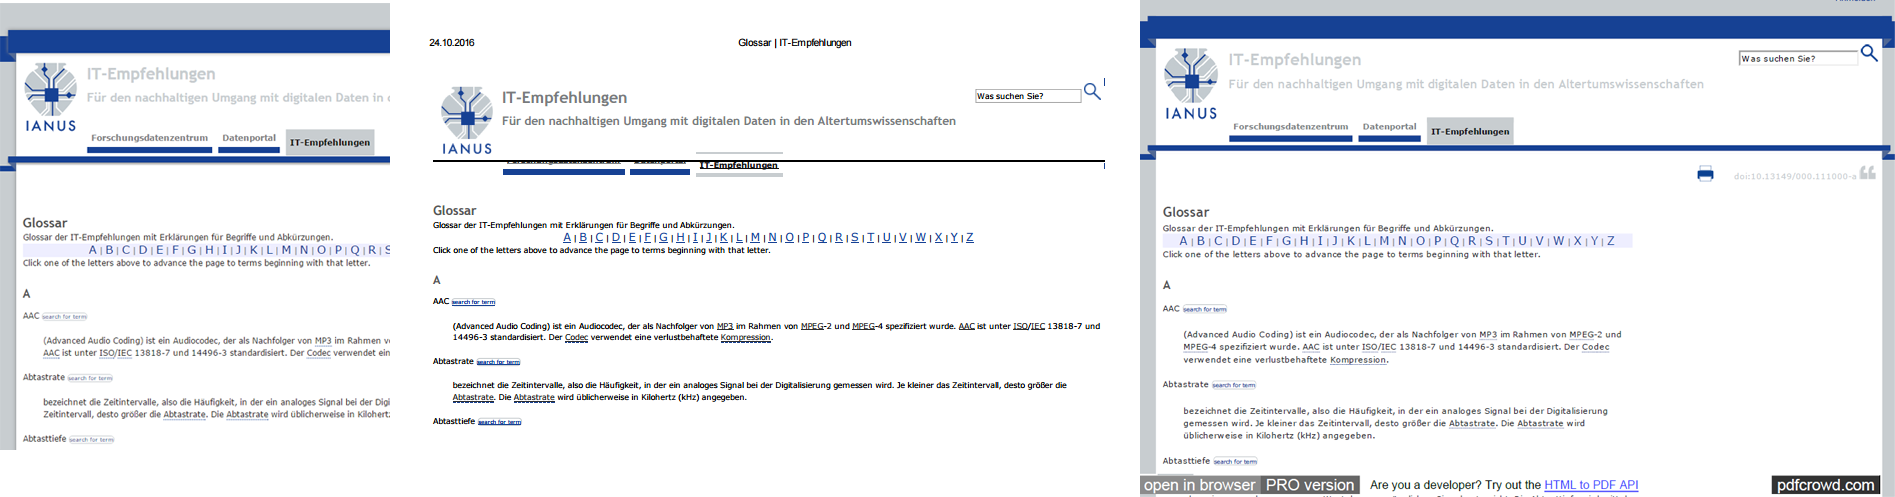
\includegraphics[width=1\textwidth]{bilder/web_pdf}
  \end{center}
  \caption{Das Glossar der IT-Empfehlungen als Screenshot (links), als mit dem Browser erzeugte PDF-Datei (mitte) und als mittels dem "`Save as PDF"'-Plug-in erzeugtes PDF (rechts).}
\end{figure}

Spezielle (kommerzielle) Programme wie die Literaturverwaltungssoftware Citavi beherrschen ebenso das Speichern von Webseiten unter Beibehaltung des Layouts als PDF. Auch bietet etwa Adobe Acrobat Pro DC eine Option zur Konvertierung von Webseiten in ein PDF-Dokument.

\begin{flushleft}
	Mozilla Firefox "`Firefox Web2PDF Converter"': \urllist{https://addons.mozilla.org/en-US/firefox/addon/web2pdf-converter}
	Mozilla Firefox "`Save as PDF"': \urllist{https://addons.mozilla.org/de/firefox/addon/save-as-pdf}
	Mozilla Firefox "`FireShot"': \urllist{https://addons.mozilla.org/de/firefox/addon/fireshot}
	Google Chrome "`Save as PDF"': \urllist{https://chrome.google.com/webstore/detail/save-as-pdf/kpdjmbiefanbdgnkcikhllpmjnnllbbc}
	Google Chrome "`FireShot"': \urllist{https://chrome.google.com/webstore/detail/capture-webpage-screensho/mcbpblocgmgfnpjjppndjkmgjaogfceg}
	Web2PDF: \urllist{http://www.web2pdfconvert.com}
	Swiss Academic Software Citavi: \urllist{https://www.citavi.com/de/index.html}  
	Adobe Acrobat Pro DC: \urllist{https://acrobat.adobe.com/at/de/acrobat.html}
\end{flushleft}


\subparagraph{Archivierung als MHTML}

MHTML-Dateien können mit Webbrowsern erstellt und geöffnet werden. Auch mit Texteditoren können MHTML-Dateien angesehen werden. Jedoch benötigen Firefox und Safari noch ein Plug-in. Bei den Webbrowsern Chrome und Vivaldi muss zuvor MHTML in den experimentellen Funktionen aktiviert werden: Bei Chrome wird hierfür \emph{chrome://flags/}, bei Vivaldi \emph{vivaldi://flags} in die Adresszeile eingegeben und die entsprechende Funktion aktiviert. Ein Neustart des Webbrowsers wird danach benötigt. Im Head der MHTML-Dateien können Metadaten mittels eines Texteditors eingetragen werden. Der Inhalt wie auch das Layout und alle Hyperlinks werden bei MHTML-Dateien in der Regel vollständig übernommen. 

\begin{figure}[h!tb]
  \begin{center}
    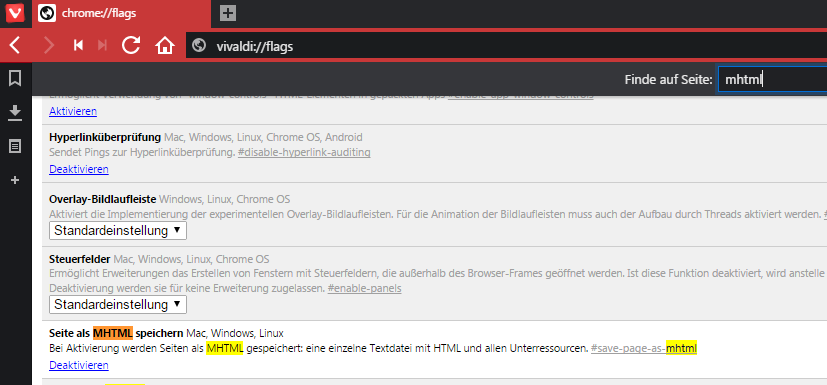
\includegraphics[width=0.95\textwidth]{bilder/web_vivaldi}
  \end{center}
  \caption{Einstellungen im Webbrowser Vivaldi}
\end{figure}

\begin{figure}[h!tb]
  \begin{center}
    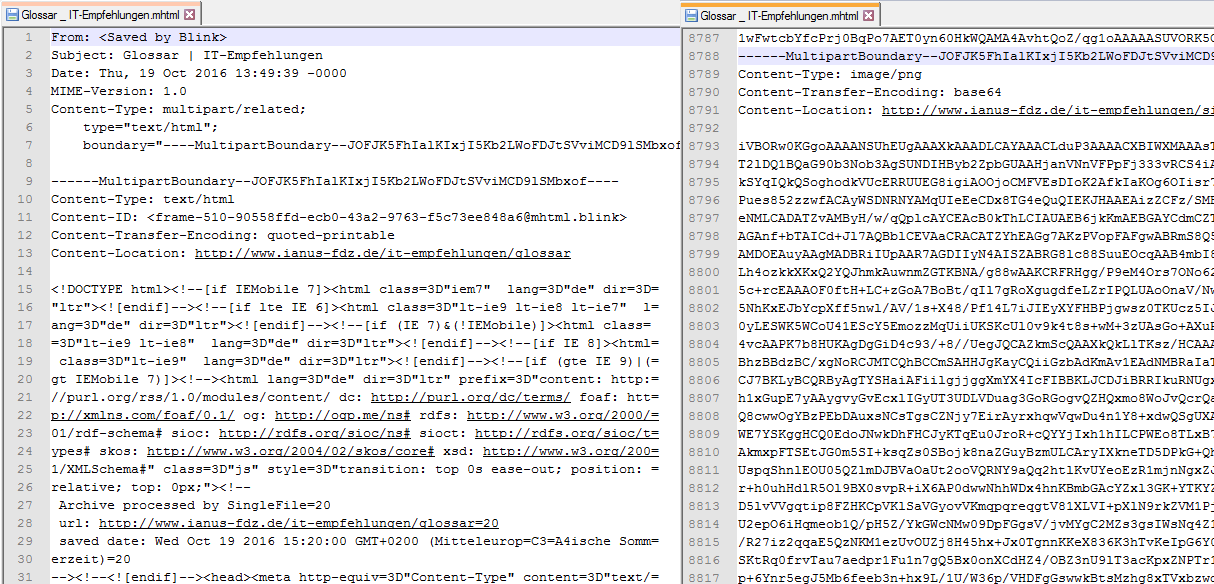
\includegraphics[width=0.95\textwidth]{bilder/web_mhtml}
  \end{center}
  \caption{Der Quellcode einer MHTML-Datei. Rechts ist der Code einer eingebetteten Grafik zu sehen.}
\end{figure}


\begin{flushleft}
	Google Chrome "`Archiveror"': \urllist{https://chrome.google.com/webstore/detail/archiveror/cpjdnekhgjdecpmjglkcegchhiijadpb}
	Google Chrome "`Save As MHTML"': \urllist{https://chrome.google.com/webstore/detail/save-as-mhtml/eomfifclcdpkaghkehajpolkdnkmegfa}
	Google Chrome "`In Google Drive speichern"': \urllist{https://chrome.google.com/webstore/detail/save-to-google-drive/gmbmikajjgmnabiglmofipeabaddhgne}
	Mozilla Firefox "`Mozilla Archive Format, with MHT and Faithful Save"': \urllist{https://addons.mozilla.org/de/firefox/addon/mozilla-archive-format}
\end{flushleft}


\subparagraph{Archivierung als MAFF-Datei}

Die Speicherung einer Webseite als MAFF-Datei wird derzeit nur von Mozilla Firefox mittels des Plug-ins "`Mozilla Archive Format, with MHT and Faithful Save"' unterstützt. MAFF-Dateien können nur von Mozilla Firefox mit diesem Plug-in geöffnet werden. Alle weiteren, aktuellen Webbrowsern können MAFF\_Dateien öffnen, indem sie mittels eines Datenkompressionsprogramms entpackt werden.
 

\begin{flushleft}
	Mozilla Firefox "`Mozilla Archive Format, with MHT and Faithful Save"': \urllist{https://addons.mozilla.org/de/firefox/addon/mozilla-archive-format}
\end{flushleft}


\subparagraph{Archivierung als HTML mit Data-URI}

Alle aktuellen Webbrowser können HTML-Dateien mit Data-URIs öffnen. Derzeit beherrscht nur der Webbrowser Google Chrome die Speicherung von Webseiten als HTML-Dateien mit Data-URIs mittels des Plug-ins "`SingleFile"'. Eine alte Version des gleichen Plug-ins existiert auch für frühere Versionen des Webbrowsers Opera.  Im Head der HTML-Dateien mit Data-URLs können Metadaten mittels eines Texteditors eingetragen werden. Der Inhalt wie auch das Layout und alle Hyperlinks werden bei HTML-Dateien mit Data-URIs in der Regel vollständig übernommen.

\begin{figure}[h!tb]
  \begin{center}
    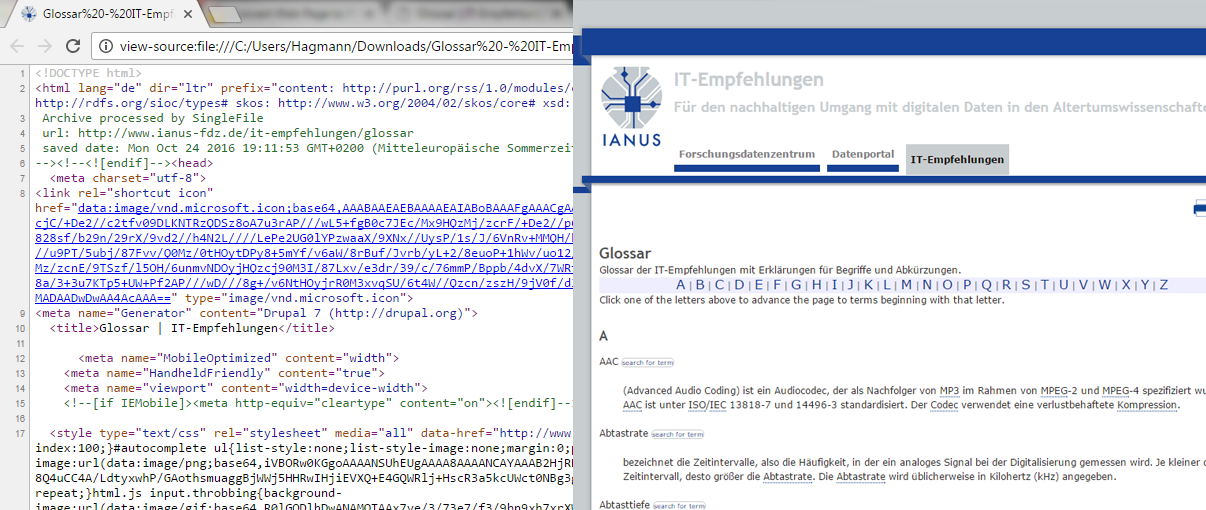
\includegraphics[width=0.95\textwidth]{bilder/web_datauri}
  \end{center}
  \caption{Links der Quellcode einer HTML-Datei mit Data-URIs. Rechts die Darstellung im Browser. Eindeutig erkennbar ist die vollständige Übernahme des Inhalts samt der Hyperlinks sowie die vollständige Übernahme des Designs. Der blau unterstrichene Codeblock ist eine Data-URI eines Bildes.}
\end{figure}


\begin{flushleft}
	Google Chrome "`SingleFile"': \urllist{https://chrome.google.com/webstore/detail/mpiodijhokgodhhofbcjdecpffjipkle}
\end{flushleft}

\subparagraph{Archivierung von Websites}
Webseiten können durch Websitearchivierungsdienste archiviert werden, wie sie durch die Bayerische Landesbibliothek (auf Antrag) oder Internet Archive angeboten werden. Dabei erfolgt die Speicherung einer Webseite auf einem Server dieser Dienste und kann über das Internet abgerufen werden. Man gibt dazu die URI der zu archivierenden Seite  bei dem Archivierungsdienst an und wird kurz darauf auf die archivierte Seite unter einer neuen URI weitergeleitet. Es kann sowohl die einzelne Webseite als auch die gesamte (oder ein Großteil) der gesamten Website archiviert werden. Metadaten müssen separat z.B. in Form einer XML-Datei, die auch den Link zur archivierten Seite enthält, gespeichert werden. Da Websitearchivierungsdienste wie Internet Archive das WWW auch selbstständig durchsuchen und Websites archivieren, kann die zu archivierende Webseite bereits auf dieser Plattform gesichert worden sein. Dies wird durch die Archivierungsdienste jedoch gesondert ausgewiesen und hindert nicht daran, die Webseite zusätzlich ein weiteres Mal zu archivieren. Plug-ins wie "`Archiveror"' für Google Chrome oder Mozilla Firefox ermöglichen die Archivierung einer Webseite direkt aus dem Browser heraus auf Internet Archive. 

\begin{figure}[h!tb]
  \begin{center}
    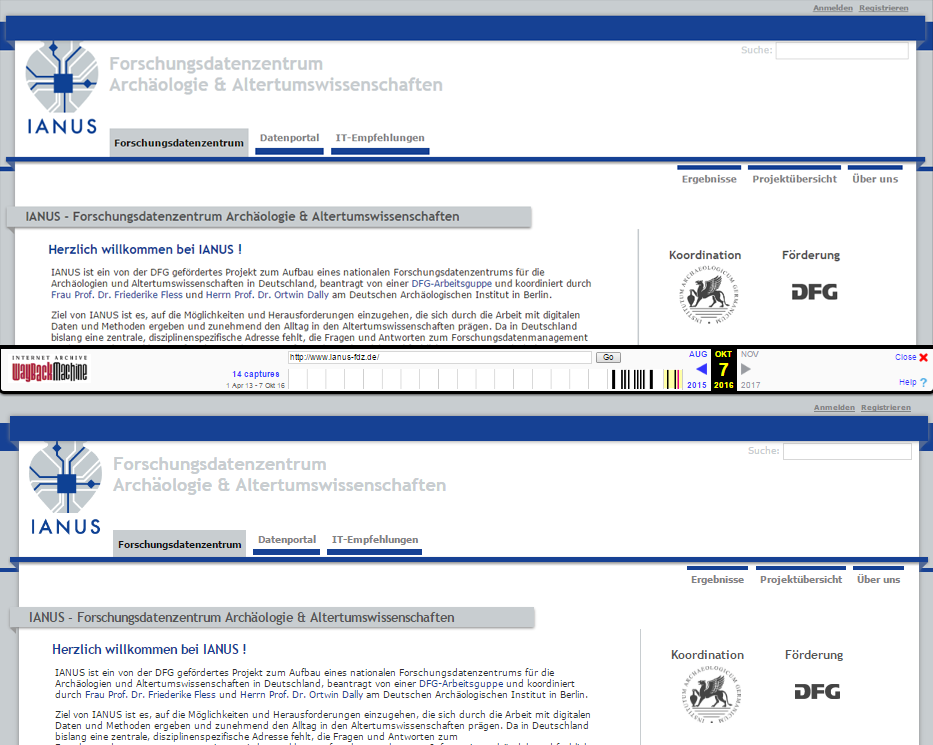
\includegraphics[width=0.95\textwidth]{bilder/web_wayback}
  \end{center}
  \caption{Screenshot der Webseite von IANUS in Google Chrome im Vollbild (oben) und ein Abbild der Webseite auf Internet Archive. Eindeutig erkennbar ist die vollständige Übernahme des Inhalts samt der Hyperlinks sowie die vollständige Übernahme des Designs.}
\end{figure}

Dezidierte Softwarelösungen wie Wget oder Heritrix ermöglichen den automatisierten Abruf aller zu einer Website gehörenden Komponente. Sie wurden primär für Linux entwickelt, können aber auch auf anderen Betriebssystemen verwendet werden. Beide sind frei verfügbar und können die gefundenen Ressourcen als WARC-Datei speichern.  

\begin{flushleft}
	Google Chrome "`Archiveror"': \urllist{https://chrome.google.com/webstore/detail/archiveror/cpjdnekhgjdecpmjglkcegchhiijadpb}
	Mozilla Firefox "`Archiveror"': \urllist{https://addons.mozilla.org/en-US/firefox/addon/archiveror}
	Dienst der Bayrischen Landesbibliothek: \urllist{https://www.babs-muenchen.de/index.html?c=workflows_web} 
	Internet Archive mit Wayback Machine: \urllist{https://archive.org/web}
	Wget: \urllist{https://www.gnu.org/software/wget}
	Heritrix: \urllist{https://webarchive.jira.com/wiki/display/Heritrix/Heritrix}
\end{flushleft}


\subparagraph{Screenshots von Webseiten}
Die Speicherung von Webseiten in der Form von Screenshots ist nicht für die Archivierung geeignet, ist aber ein gutes Hilfsmittel, um das ursprüngliche Aussehen der Webseite zu dokumentieren. Screenshots können mit Hilfe der Screenshot-Funktion des Computers, spezieller Screenshot Software (z.B. Microsofts Snipping Tool) oder durch eigene, auf die Verarbeitung von Webseiten spezialisierte Plug-ins für Webbrowser erzeugt werden. Während für gewöhnlich mit der Screenshot Funktion des Computers der gesamte Bildschirm bzw. aktive Fenster und mit Screenshot Softwarelösunge zusätzlich einzelne Bildauschnitte als Grafiken gespeichert werden können, fertigen erwähnte Plug-ins einen Screenshot der gesamten Webseite oder eines ausgewählten Teiles davon an. Screenshots werden durch die erwähnten Funktionen und Programme in der Regel im PNG- oder JPEG-Format gespeichert.



\paragraph{Quellen}
\begin{flushleft}
U. Ackermann -- C. Berner -- N. Elbert -- J. Kett -- K. K. Koçer -- N. von der Hude -- M. Wiegand, Policy für die Vergabe von URNs im Namensraum urn:nbn:de (2012) \urllist{http://d-nb.info/1029114455/34}

N. Brügger, Archiving Websites. General Considerations and Strategies (Aarhus 2005) \urllist{http://cfi.au.dk/fileadmin/www.cfi.au.dk/publikationer/archiving_underside/archiving.pdf}

Archaeology Data Service –- Digital Antiquity, Documents and Digital Texts: A Guide to Good Practice. Section 2. Creating Texts and Documents \urllist{http://guides.archaeologydataservice.ac.uk/g2gp/TextDocs_2}

Archaeology Data Service –- Digital Antiquity, Documents and Digital Texts: A Guide to Good Practice. Section 3. Archiving Texts and Documents \urllist{http://guides.archaeologydataservice.ac.uk/g2gp/TextDocs_3}

DOI (Hrsg.), DOI Handbook \urllist{https://www.doi.org/hb.html}

A. Rauber -- H. Liegmann, Webarchivierung zur Langzeiterhaltung von Internet-Dokumenten, in: H. Neuroth -- A. Oßwald -- R. Scheffel -- S. Strathmann -- K. Huth (Hrsg.) nestor Handbuch. Eine kleine Enzyklopädie der digitalen Langzeitarchiverung. Version 2.3 (2010) Kap. 17.9 \urllist{http://www.nestor.sub.uni-goettingen.de/handbuch}

S. M. Schafer, HTML, XHTML, and CSS Bible \textsuperscript{4}(Indianapolis 2008)\abstand

M. Schäfer, Einführung in JavaScript – Deutschsprachige Dokumentation der Programmiersprache JavaScript \urllist{http://molily.de/js/} 

SELFHTML-Wiki, Glossar \urllist{https://wiki.selfhtml.org/wiki/Kategorie:Glossar}

M. Trognitz, Abschlussbericht Testbed "`Persistent Identifiers"' (2013) \urllist{http://www.ianus-fdz.de/attachments/download/560/Testbed-Persistent\%20Identifiers.pdf}

W3C (Hrsg.), CSS \urllist{https://www.w3.org/Style/CSS}

W3C (Hrsg.), DOM \urllist{https://www.w3.org/DOM}

W3C (Hrsg.), HTML \urllist{https://www.w3.org/html}

W3C \urllist{https://www.w3c.org}

W3schools \urllist{http://www.w3schools.com/default.asp}


\quelltyp{Formatspezifikationen}
HTML: \urllist{https://www.w3.org/TR/html5}
XHTML: \urllist{https://www.w3.org/TR/html5}
CSS: \urllist{https://www.w3.org/TR/2011/REC-CSS2-20110607}
MHTML: RFC 2557 \urllist{https://tools.ietf.org/html/rfc2557}
WARC 0.9: \urllist{http://archive-access.sourceforge.net/warc/warc_file_format-0.9.html}
WARC: ISO 28500 \urllist{http://www.iso.org/iso/iso_catalogue/catalogue_tc/catalogue_detail.htm?csnumber=44717}
WARC: Library of Congress \urllist{http://www.digitalpreservation.gov/formats/fdd/fdd000236.shtml}
MAFF: \urllist{http://maf.mozdev.org/maff-specification.html}
Data-URI: RFC 2397 \urllist{https://tools.ietf.org/html/rfc2397} 
WWW: RFC 7540 \urllist{https://tools.ietf.org/html/rfc7540} 
FTP: RFC 959 \urllist{https://tools.ietf.org/html/rfc959}
HTTP: RFC 7540 \urllist{https://tools.ietf.org/html/rfc7540}
HTTP: \urllist{https://html.spec.whatwg.org/multipage}
URI, URL : RFC 3986 \urllist{https://tools.ietf.org/html/rfc3986}
URN: RFC 2141 \urllist{https://tools.ietf.org/html/rfc2141}
Java: \urllist{https://docs.oracle.com/javase/specs}
Java: \urllist{http://docs.oracle.com/javase/specs/jls/se8/html/index.html}
JavaScript: \urllist{http://www.ecma-international.org/ecma-262/5.1}
JavaScript: \urllist{http://ecma-international.org/ecma-402/1.0/index.html}


\quelltyp{Tools und Programme}
	Adobe Muse CC: \urllist{https://www.adobe.com/at/products/muse.html}
	Adobe Dreamweaver CC: \urllist{https://www.adobe.com/at/products/dreamweaver.html}
	Sublime Text: \urllist{https://www.sublimetext.com}
	Aptana Studio: \urllist{http://www.aptana.com}
	Seamonkey: \urllist{http://www.seamonkey-project.org}
	BlueGriffon: \urllist{http://www.bluegriffon.org}
	Mozilla Firefox "`Firefox Web2PDF Converter"': \urllist{https://addons.mozilla.org/en-US/firefox/addon/web2pdf-converter}
	Mozilla Firefox "`Save as PDF"': \urllist{https://addons.mozilla.org/de/firefox/addon/save-as-pdf}
	Mozilla Firefox "`FireShot"': \urllist{https://addons.mozilla.org/de/firefox/addon/fireshot}
	Google Chrome "`Save as PDF"': \urllist{https://chrome.google.com/webstore/detail/save-as-pdf/kpdjmbiefanbdgnkcikhllpmjnnllbbc}
	Google Chrome "`FireShot"': \urllist{https://chrome.google.com/webstore/detail/capture-webpage-screensho/mcbpblocgmgfnpjjppndjkmgjaogfceg}
	Web2PDF: \urllist{http://www.web2pdfconvert.com}
	Swiss Academic Software Citavi: \urllist{https://www.citavi.com/de/index.html}  
	Adobe Acrobat Pro DC: \urllist{https://acrobat.adobe.com/at/de/acrobat.html}
	Google Chrome "`Archiveror"': \urllist{https://chrome.google.com/webstore/detail/archiveror/cpjdnekhgjdecpmjglkcegchhiijadpb}
	Mozilla Firefox "`Archiveror"': \urllist{https://addons.mozilla.org/en-US/firefox/addon/archiveror}
	Google Chrome "`Save As MHTML"': \urllist{https://chrome.google.com/webstore/detail/save-as-mhtml/eomfifclcdpkaghkehajpolkdnkmegfa}
	Google Chrome "`In Google Drive speichern"': \urllist{https://chrome.google.com/webstore/detail/save-to-google-drive/gmbmikajjgmnabiglmofipeabaddhgne}
	Mozilla Firefox "`Mozilla Archive Format, with MHT and Faithful Save"': \urllist{https://addons.mozilla.org/de/firefox/addon/mozilla-archive-format}
	Dienst der Bayrischen Landesbibliothek: \urllist{https://www.babs-muenchen.de/index.html?c=workflows_web} 
	Internet Archive mit Wayback Machine: \urllist{https://archive.org/web}
	Wget: \urllist{https://www.gnu.org/software/wget}
	Heritrix: \urllist{https://webarchive.jira.com/wiki/display/Heritrix/Heritrix}
\end{flushleft}